\documentclass{standalone}
% Set target color model to RGB
\usepackage[rgb]{xcolor}
\usepackage{tikz}
\begin{document}
	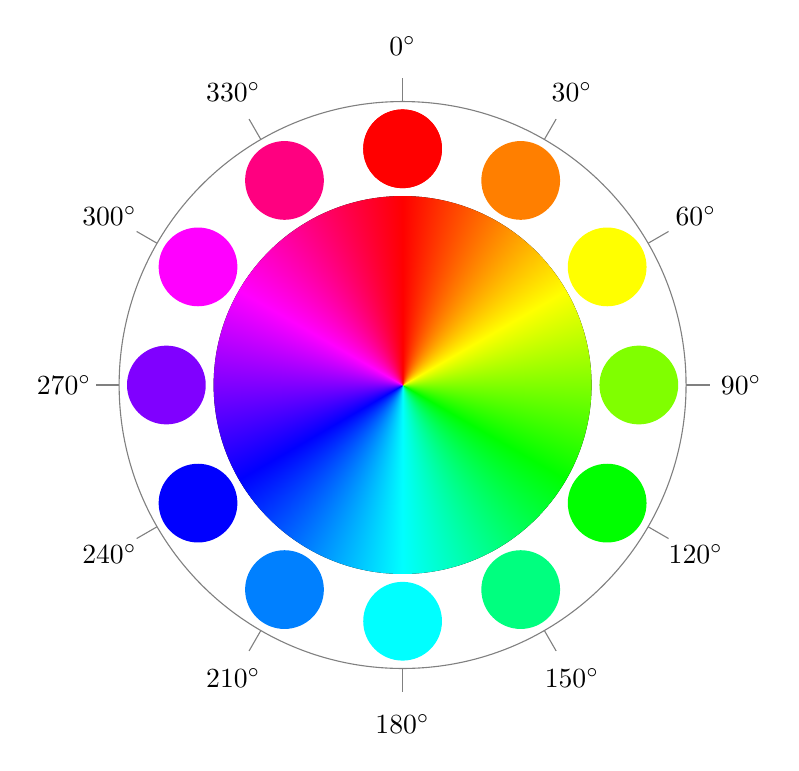
\begin{tikzpicture}
		% Hệ màu HSB = HSV
		% H = hue = sắc độ
		\foreach \i in {0,30,...,360} {
			\pgfmathsetmacro{\ih}{\i/360}
			\definecolor{currentcolor}{hsb}{\ih,1,1}
			\fill[currentcolor] (-\i+90:3) circle(.5);
		}
		% Bánh xe màu sắc
		\usepgflibrary{shadings}
		\fill[shading=color wheel] (0,0)circle(2.4);
		\draw[gray] (0,0) circle(3.6);
		\foreach \i in {0,30,...,330}
		\draw[gray] (-\i+90:3.6)--(-\i+90:3.9)
		(-\i+90:4.3) node[black]{$\i^\circ$};
	\end{tikzpicture}
\end{document}